\documentclass{article}
\usepackage[utf8]{inputenc}
\usepackage{tikz}
\usepackage{acro}
\usepackage{graphicx}
\usepackage{amsmath}
\usepackage[colorlinks=true, urlcolor=blue]{hyperref}

% Define acronyms
\DeclareAcronym{API}{short=API, long=Application Programming Interface}
\DeclareAcronym{GUI}{short=GUI, long=Graphical User Interface}

\title{tex2docx Demo Document}
\author{tex2docx Project}
\date{\today}

\begin{document}

\maketitle
\newpage

\tableofcontents
\newpage

\printacronyms[name=List of Acronyms]
\newpage

\section{Introduction}
This is a sample document to demonstrate the capabilities of \texttt{tex2docx}. It includes a title page, table of contents, acronyms, TikZ figures, and a bibliography.

\subsection{Acronyms}
Here we use some acronyms. The \ac{API} allows different software components to communicate. Users interact with the system through the \ac{GUI}. We can also use plural forms like \acp{API}.

\section{TikZ Diagrams}
One of the main features is converting TikZ diagrams into high-resolution images. Below is a simple block diagram.

\begin{figure}[h!]
\centering
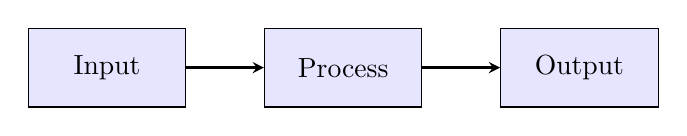
\begin{tikzpicture}[
    box/.style={draw, rectangle, minimum width=2cm, minimum height=1cm, fill=blue!10},
    arrow/.style={thick, ->, >=stealth}
]
    \node[box] (input) at (0,0) {Input};
    \node[box] (process) at (3,0) {Process};
    \node[box] (output) at (6,0) {Output};

    \draw[arrow] (input) -- (process);
    \draw[arrow] (process) -- (output);
\end{tikzpicture}
\caption{A simple process diagram.}
\end{figure}

\section{Equations}
Standard LaTeX math environments are fully supported and converted seamlessly into Word equations.

Here is an inline equation: $E = mc^2$. And here is a block equation:
\begin{equation}
    f(x) = \int_{-\infty}^{\infty} \hat{f}(\xi)\,e^{2 \pi i \xi x} \,d\xi
\end{equation}

You can also use aligned equations:
\begin{align}
    a^2 + b^2 &= c^2 \\
    \sin^2 \theta + \cos^2 \theta &= 1
\end{align}

\section{Formatting}
Standard LaTeX formatting is preserved:
\begin{itemize}
    \item \textbf{Bold text} for emphasis.
    \item \textit{Italic text} for terms.
    \item URLs like \url{https://github.com/scavero/tex2docx}.
\end{itemize}

\section{Conclusion}
This tool makes it easy to convert LaTeX to Word, especially when using complex packages like TikZ. For more details, see \cite{lamport94}.

\newpage
\begin{thebibliography}{99}
\bibitem{lamport94}
  Leslie Lamport,
  \textit{\LaTeX: A Document Preparation System}.
  Addison Wesley, Massachusetts,
  2nd Edition,
  1994.

\bibitem{mittelbach04}
  Frank Mittelbach, Michel Goossens,
  \textit{The \LaTeX{} Companion}.
  Addison-Wesley,
  2nd Edition,
  2004.
\end{thebibliography}

\end{document}
